\documentclass[12pt, aspectratio=169]{beamer} % aspectratio = 43 of 169
\usepackage{color}
\usepackage{graphicx}
\usepackage{tikz}
\usepackage{transparent}

% kleuren (theme=...): red (standaard), blue, cyan, orange, green
% official=false: een mooie, maar niet-officiele stijl
% official=true: de stijl die ze ook in PowerPoint hebben, met dat blauwe blokje onderaan
% MERK OP: bij official=true is de nummering van de slides verkeerd!
\usetheme[department=winuk,official=false,theme=cyan,innovation=false,titlebgimage=imgs/screenshot-titleframe.png]{tue2008}

\mode<presentation>

\setbeamercolor{alerted text}{fg=tueblue}

\graphicspath{{./imgs}}

% http://stackoverflow.com/a/5971923/962603
\newenvironment{animationframe}
  {\begin{frame}}
  {\end{frame} \addtocounter{framenumber}{-1}}

\title{Building a conveyor belt editor and simulator}
\author{Thom Castermans and Willem Sonke}

\begin{document}

\begin{titleframe}
\end{titleframe}

\begin{frame}
  \transduration<1>{3}
  \frametitle{Project idea}
  \begin{columns}[c]
    \column{.6\textwidth}
      \begin{itemize}
        \item Block editor\uncover<2->{\ldots\ with a twist!
        \item Building a conveyor belt system
        \item Simulating luggage movement}
      \end{itemize}
    \column{.4\textwidth}
      \uncover<2->{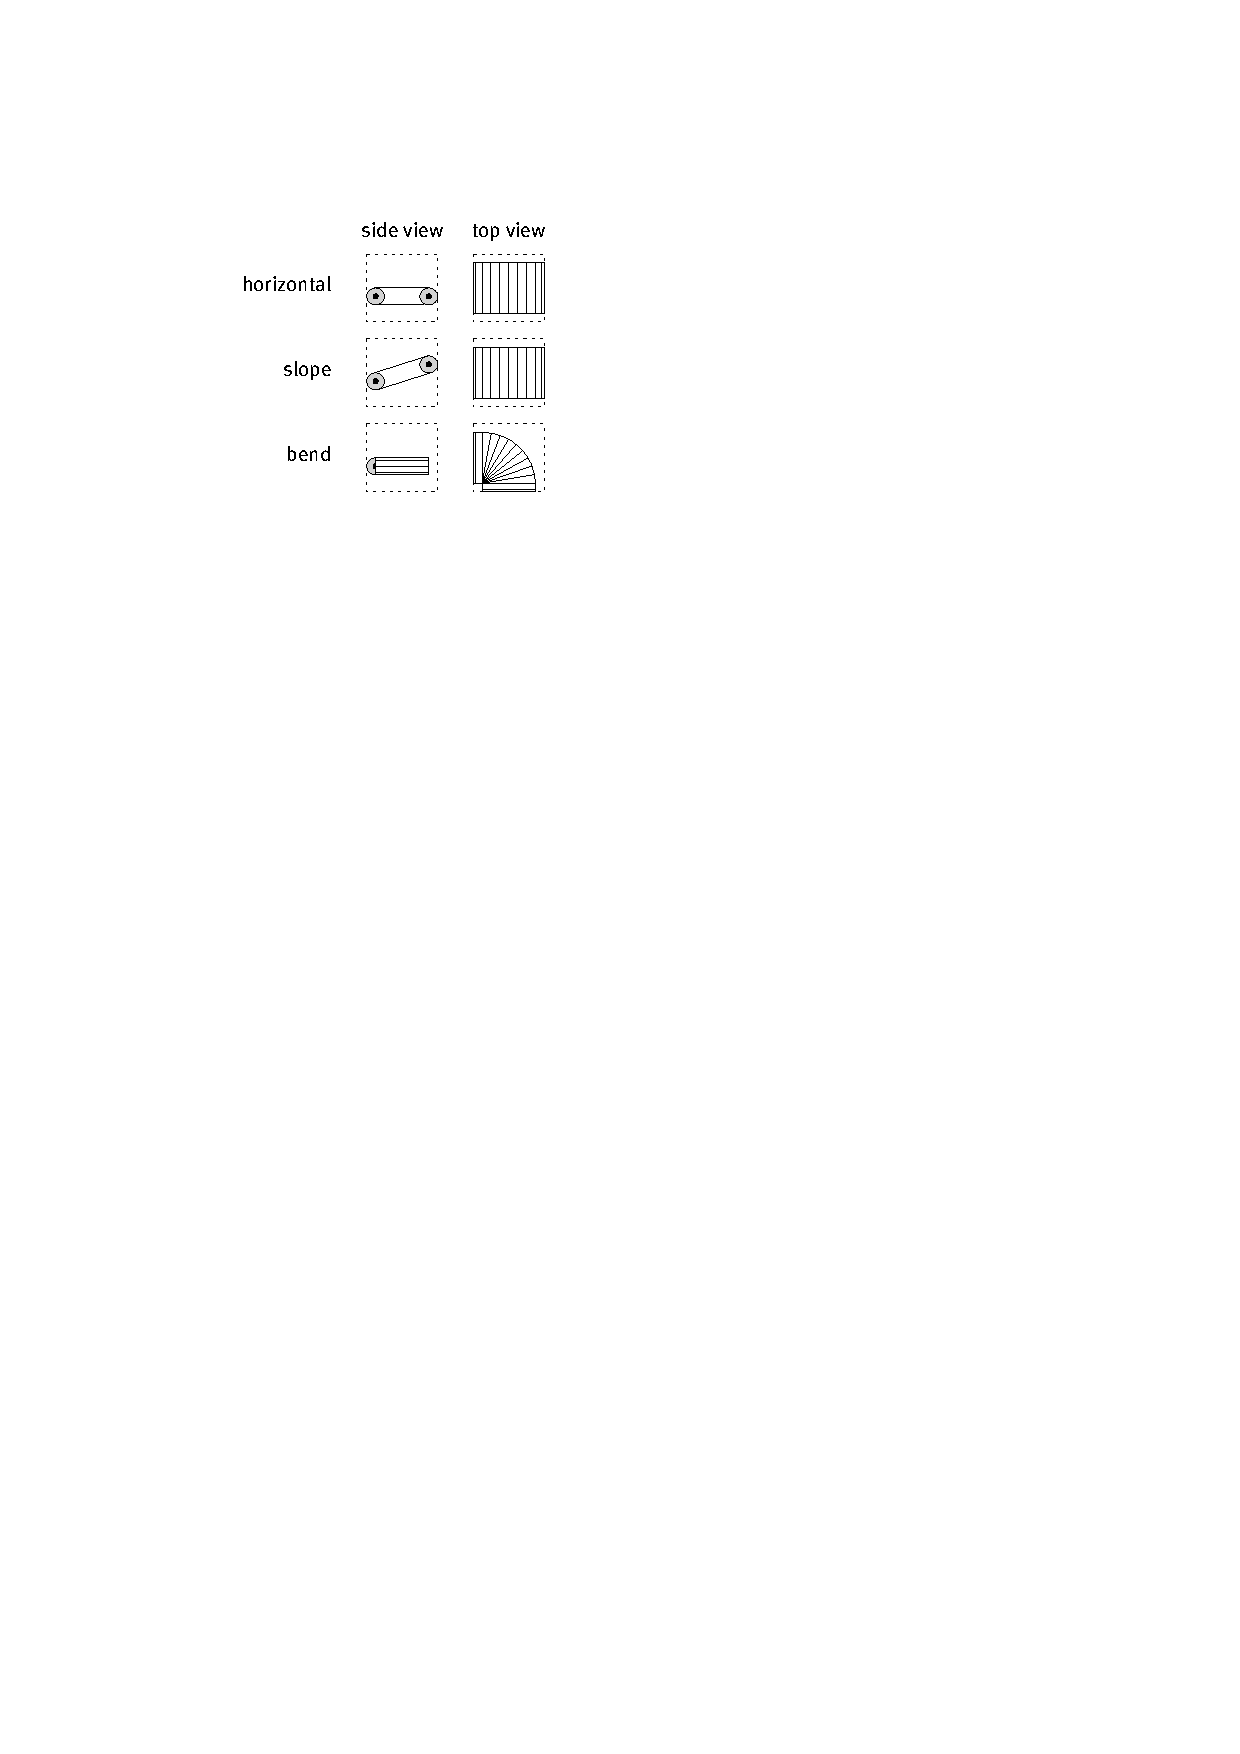
\includegraphics{imgs/sketch-blocks}}
  \end{columns}
\end{frame}

\begin{frame}
  \frametitle{Requirements}
  \begin{itemize}
    \item Very intuitive interface
    \begin{itemize}
      \item new users can easily find the functionality
    \end{itemize}
    \item Efficient interface
    \begin{itemize}
      \item frequent tasks can be executed quickly by the user
    \end{itemize}
  \end{itemize}
\end{frame}

\begin{frame}[<+->]
  \frametitle{Work so far}
  \begin{itemize}
    \item Using LWJGL to access OpenGL from Java
    \item Building a GUI in OpenGL
    \item Intuitive camera control
    \item Animating conveyor belts
    \item Initial simulation
  \end{itemize}
\end{frame}

\begin{frame}
  \frametitle{Problems\,/\,solutions}
  \begin{itemize}
    \item Drawing\,/\,texturizing the conveyor belts
    \begin{itemize}
      \item want to texturize without deformation
      \item however, different shapes of conveyor belts
    \end{itemize}
  \end{itemize}
  \begin{center}
    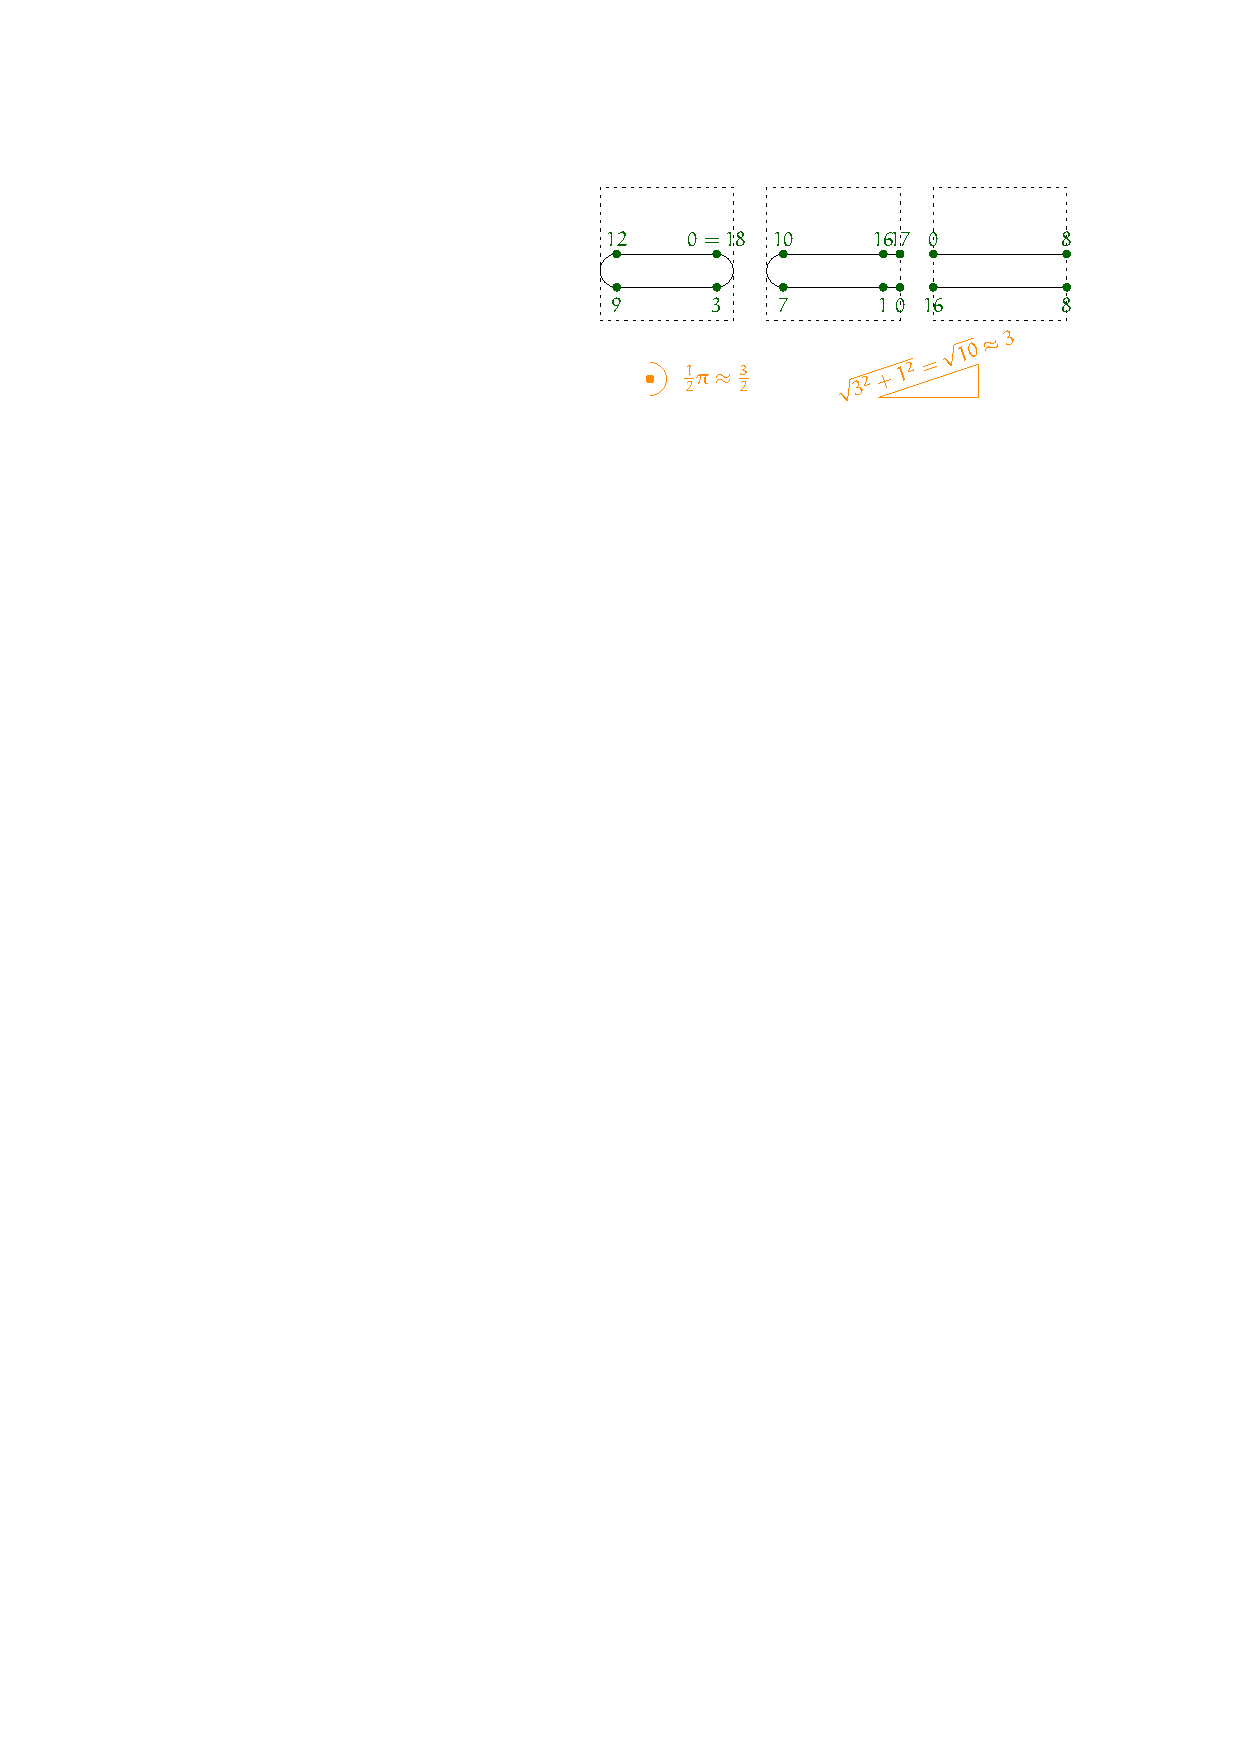
\includegraphics{imgs/sketch-texturing} % TODO [ws] graphics path doesn't seem to work? Hardcoded imgs for now
  \end{center}
\end{frame}

\begin{frame}
  \frametitle{Planned work}
  \begin{columns}[c]
    \column{.67\textwidth}
      \begin{itemize}
        \uncover<1->{
        \item Drawing adjacent conveyor belts connected
        }
        \uncover<2->{
        \item Improving simulation
        }
        \uncover<3->{
        \item Actual editing\ldots
        }
        \uncover<4->{
        \item Adding scanners
        }
        \uncover<5->{
        \item Game-like experience, with levels
        }
        \uncover<6->{
        \item ``Sandbox mode''
        }
      \end{itemize}
    \column{.33\textwidth}
      \uncover<1>{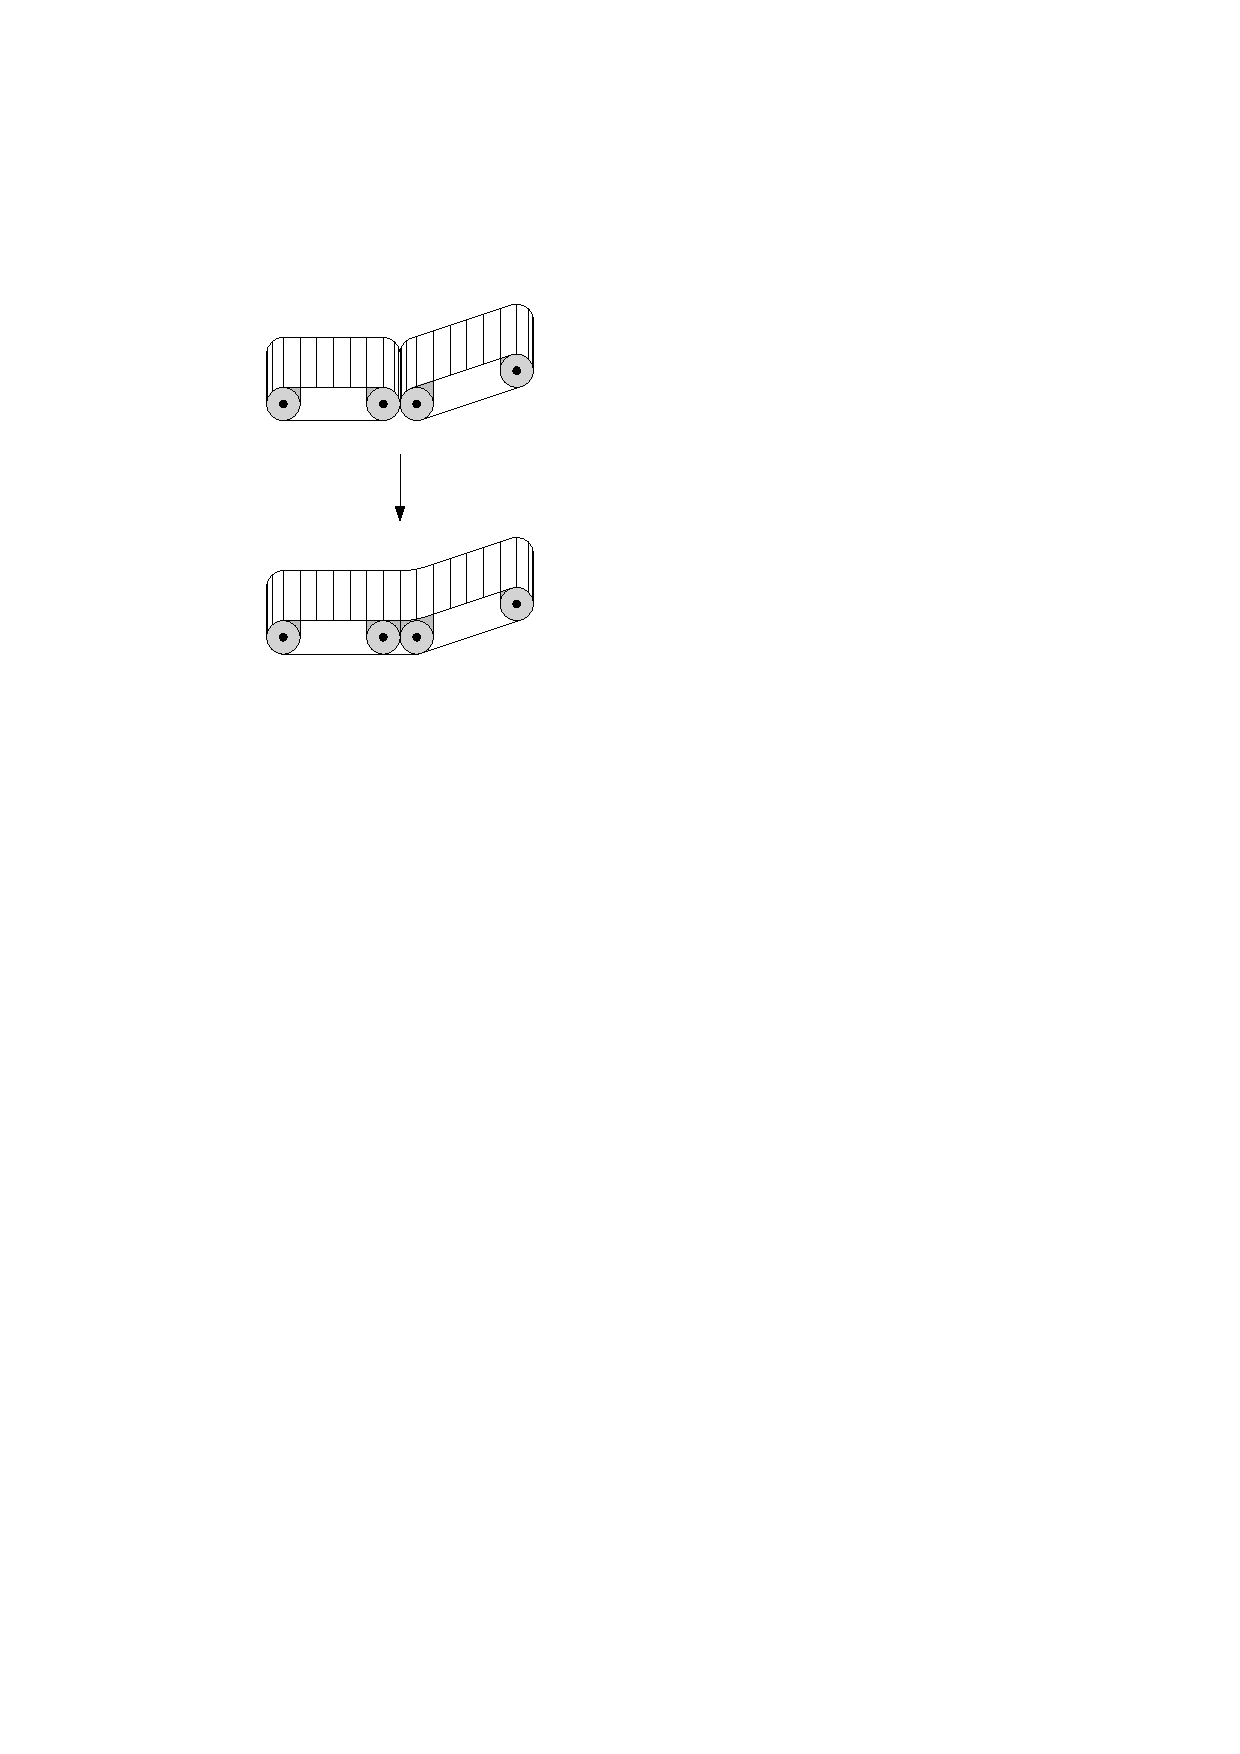
\includegraphics{imgs/sketch-adjacent-blocks}}
  \end{columns}
\end{frame}

% this does not use the graphicspath... weird
\usebackgroundtemplate{
\includegraphics[width=\paperwidth,height=\paperheight]{imgs/demo-background-011.jpg}}
\begin{frame}
  \transduration{0.25}
  \transparent{1.0}
  \begin{center}\huge\alert{Demo time!}\end{center}
\end{frame}

% generate animation frames using a for-each loop
\foreach \transparency / \filename in {0.9/010, 0.8/009, 0.7/008, 0.6/007, 0.5/006, 0.4/005, 0.3/004, 0.2/003, 0.1/002, 0.0/001} {
\usebackgroundtemplate{\includegraphics[width=\paperwidth,height=\paperheight]{imgs/demo-background-\filename.jpg}}
\begin{animationframe}
  \transduration{0.25}
  \transparent{\transparency}
  \begin{center}\huge\alert{Demo time!}\end{center}
\end{animationframe}
}

\end{document}
